\sectionlink{まとめと展望}
\label{section:Summary}

本論文では、非平衡開放系における時間並進対称性の破れに対応する有効場理論を構築する一般的な方法を定式化した。最も簡単な例であるBrown運動を用いて、時間並進の自発的対称性の破れ（SSB）に対する\textit{弱い}判定基準などの基本概念を導入した後、Schwinger-Keldysh形式における二重化された時間並進対称性の構造に基づいて、一般的な状況でEFTを構築するための確かな基礎を与えた。得られたEFTを用いれば、開放系における対応するNGモードとギャップを持つモードの分散関係を求めることができる。最も一般的な有効Lagrangianを構成した後、系の熱的性質の名残とみなせる動的KMS対称性に由来する、低エネルギー（Wilson）係数に対する非自明な制約も議論した。

\medskip
本定式化を適用できる非平衡系は、宇宙論、物性物理学、化学系など多岐にわたり、生物系や経済系にも適用できる可能性がある。有望な応用の一つは、初期宇宙のインフレーションに対する開放系EFTの構築である。本論文では平坦空間の力学に焦点を当てたが、議論を曲がった時空へ拡張することは容易であろう。これは、いわゆる宇宙論的コライダー物理の研究計画~\cite{Chen:2009zp,Baumann:2011nk,Noumi:2012vr,Arkani-Hamed:2015bza}を補完する手法として、インフレーション期の隠れたセクターの粒子を探るのに役立つであろう。また、例えば確率的インフレーション~\cite{stochastic}や温かいインフレーション~\cite{Berera:1995ie}に対し、模型に依存しない枠組みを与えることにもなる。

\medskip
もう一つの興味深い方向は、冷却原子系などの物性物理学への応用である。実際、駆動散逸型の冷却原子系には、非平衡相転移と、それに対応する新たな対称性の破れた相が存在することが最近指摘されている~\cite{PhysRevLett.96.230602,PhysRevLett.99.140402,sieberer2016keldysh}。興味深い点の一つは、いくつかの模型が時間依存する凝縮を示すことである。これは\textit{強い}意味での時間並進対称性の自発的破れとみなせる（SSBに対する本論文の\textit{弱い}および\textit{強い}判定基準については脚注\ref{footnote4}を参照）。ただし、例えば$U(1)$対称性に伴う振動する凝縮がある場合、その状態は時間並進と大域的$U(1)$変換を組み合わせた変換の下で対称なままであることに注意したい。その場合、この対称性の破れは$U(1)$対称性の破れとしても、時間並進対称性の破れとしても捉えられる。したがって、そのような系を記述するうえでどちらの記述がより適切かを明らかにする必要がある。

\medskip
本形式を化学系や生物系に応用できる可能性もある。実際、同期現象を示すBelousov-Zhabotinsky反応のような開放非平衡系は数多い。これもまた時間並進対称性の破れとみなすことができる。系の遅い、すなわち低エネルギーの力学を導くためには、従来、いわゆる特異摂動法が用いられてきた~\cite{Kuramoto,MoriKuramoto}。有効Lagrangianに基づく本定式化と特異摂動法は一見異なるものの、位相の力学に着目するという基本的な考え方は共通している。したがって、本形式を応用するだけでなく、同期現象を扱う従来の方法との関係を調べることも興味深いであろう。

\section*{\hyperlink{toc}{謝辞}}
\phantomsection\addcontentsline{toc}{section}{謝辞}
著者らは、有益な議論をしていただいたY. Hidaka、Y. Minami、およびPak Hang Chris Lauに感謝する。M.H.はRIKENのSpecial Postdoctoral Researchers Programの支援を受けた。S.K.はSenshu Scholarship Foundationの部分的な支援を受けている。T.N.はJSPS KAKENHIの助成番号JP17H02894およびJP18K13539、ならびにMEXT KAKENHIの助成番号JP18H04352による部分的な支援を受けている。A.O.はJSPS Overseas Research Fellowshipsの支援を受けている。本研究はRIKEN iTHEMS Program（特にiTHEMS STAMP working group）の部分的な支援を受けた。

\appendix
\renewcommand{\thesection}{\Alph{section}}
\renewcommand{\theequation}{\Alph{section}.\arabic{equation}}
\sectionlink{環境に由来する混合項の導出}\label{kim}

本付録では、式\eqref{eq:EachL}で与えられる微視的な全Lagrangian~\eqref{eq:TotalL}から出発し、環境との結合に由来するゆらぎと散逸を表す、式\eqref{eq:MSR3}の混合項の導出を概説する（詳しい議論については、例えば文献~\cite{Kamenev:2009jj}を参照）。記法を簡単にするため、$X\to M^{-1/2}X$および$x_n\to m_n^{-1/2}x_n$と再スケールし、それに対応して$g_n\to m_n^{1/2}M^{1/2}g_n$とすることにより、この節全体で正準規格化された変数を用いる。まず、環境が一つの調和振動子からなる最も簡単な状況を考え、その後で議論を複数の振動子の場合へ一般化する。そのため、ここでは環境が初期時刻$t_0$に熱化していると仮定する。

\medskip
通常のSchwinger-Keldysh形式~\cite{Kamenev:2009jj,Bellac:2011kqa}と同様に、まず閉時間経路（CTP）の積分路$C = \bigcup_a C_{a}~ (a=1,\cdots,4)$をパラメータ表示する関数$t = z(v)$を導入する。ここで$v$は単調増加する実パラメータであり、$\sigma$は後退経路$C_2$の虚時間方向の位置を決めるパラメータである（図\ref{app:ctp}左を参照）。このとき、CTP積分路$C$上の階段関数と$\delta$関数を次のように定義する。
\begin{align}
 \theta_{C}(t-t') &\equiv \theta( v-v' ), \\
 \delta_{C} (t-t')
 &\equiv \frac{d}{dt}\theta_{C}(t -t')
 = \left( \frac{dz}{dv} \right)^{-1} \delta(v-v'),
\end{align}
ここで$\theta(v-v')$と$\delta(t-t')$は通常の階段関数と$\delta$関数である。これらを用いて、環境の振動子の実時間2点Green関数を次のように導入する。
\begin{equation}
 \begin{split}
  G_C (t- t')
  &\equiv
  \average{T_C \big( \hx (t) \hx (t') \big)} \\
  &= \theta_C (t-t') \average{\hx (t) \hx (t')}
  + \theta_C (t'-t) \average{\hx (t') \hx (t)} \\
  &= \theta_C (t-t') G^> (t- t')
  + \theta_C (t'-t) G^< (t- t'),
 \end{split}
 \label{eq:CTPGreen}
\end{equation}
ここで$T_C$はCTP積分路$C$上の時間順序積を表す。また、任意の演算子$\hOcal$に付した山括弧は熱平均を表す。
\begin{equation}
 \average{\hOcal} \equiv
  \mathrm{Tr} \big(\hat{\rho}_{\mathrm{eq}} \hOcal \big)
  \with
  \hat{\rho}_{\mathrm{eq}}
  \equiv \frac{1}{Z} e^{-\beta \hat{H}_{\mathrm{env}}}
  ~\mathrm{and}~~
 \hat{H}_{\mathrm{env}} \equiv
  \frac{\hp^2}{2} + \frac{1}{2} \omega_0^2 \hx^2 ,
\end{equation}
$\beta$は環境の逆温度である。式\eqref{eq:CTPGreen}の最終行では、次のgreater Green関数とlesser Green関数を導入した。
\begin{equation}
  G^> (t- t') \equiv \average{\hx (t) \hx (t')}, \quad
   G^<(t- t') \equiv  \average{\hx (t') \hx (t)} ,
\end{equation}
これらは、初期状態が熱的集団であることから、KMS（Kubo-Martin-Schwinger）条件を満たす。
\begin{equation}
 G^> (t- t') = G^< (t- t'+i\beta).
\end{equation}
KMS条件により、Fourier空間でのgreater/lesser Green関数は次のように表される。
\begin{equation}
 G^> (\omega) = \big( 1 + n_B (\omega) \big) \rho (\omega), \quad
  G^< (\omega) = n_B (\omega) \rho (\omega),
\end{equation}
ここで、スペクトル関数$\rho(\omega)$とBose-Einstein分布$n_B(\omega)$を次のように導入した。
\begin{equation}
 \rho (\omega) \equiv G^>(\omega) - G^< (\omega),
  \quad
  n_B (\omega) \equiv \frac{1}{e^{\beta \omega} - 1}.
\end{equation}
以下の計算では、調和振動子のスペクトル関数の具体形$\rho(\omega)=2\pi\,\mathrm{sgn}(\omega)\delta(\omega^2-\omega_0^2)$を用いる。ここで$\mathrm{sgn}(x)$は符号関数である。

\begin{figure}[t]
\begin{center}
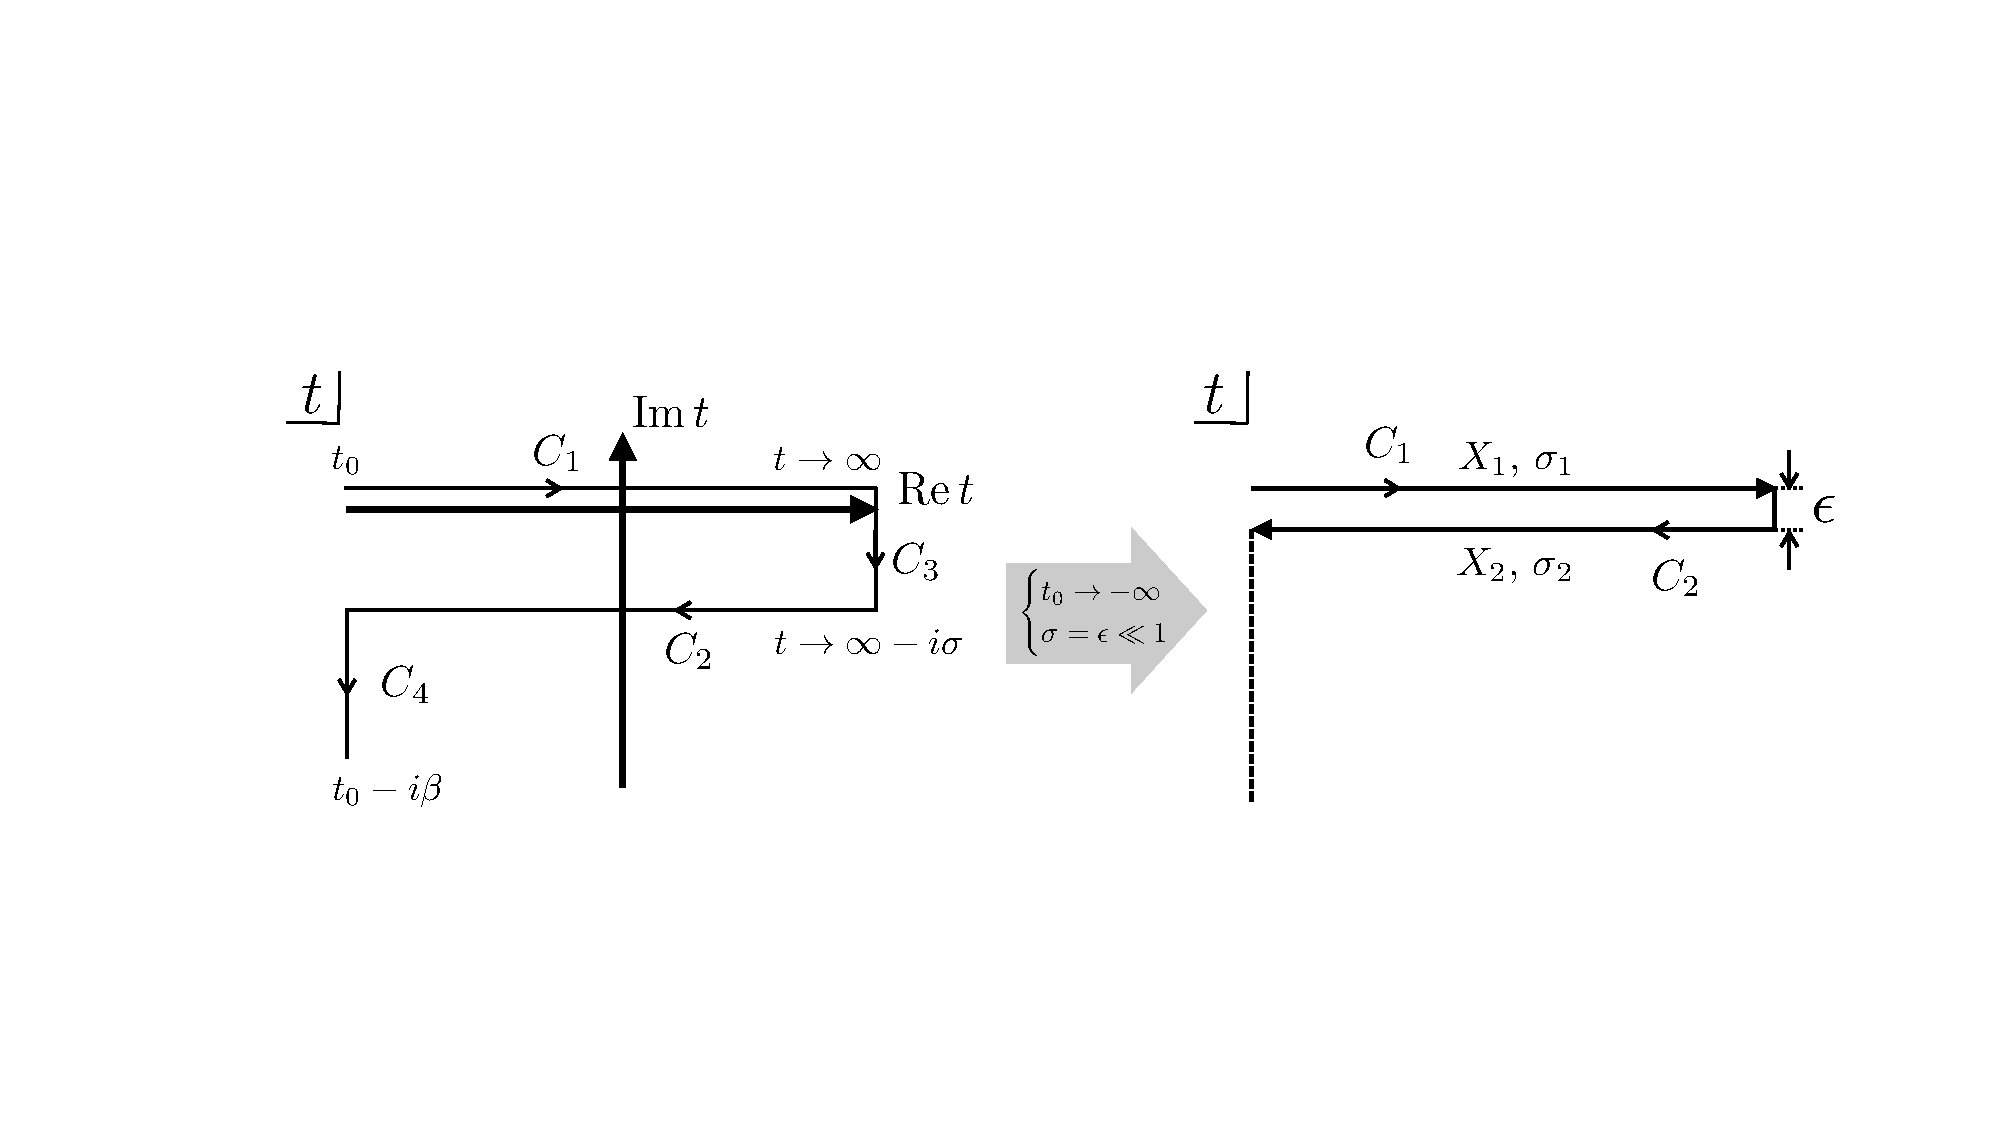
\includegraphics[width=15cm]{original/fig_ctp_ap}
\caption{初期時刻に熱化した系の一般的な閉時間経路（CTP）積分路$C$（左図）から出発し、初期時刻を過去無限遠へ移し（$t_0\to-\infty$）、前進経路と後退経路を互いに重ねる（$\sigma=\epsilon\ll1$）極限（右図）を選ぶ。この極限では、前進経路と後退経路上の変数（それぞれ$(X_1,\sigma_1)$および$(X_2,\sigma_2)$で表される）の間のGreen関数のみを考えればよい。}
\label{app:ctp}
\end{center}
\end{figure}

\medskip
系の有効作用$S_{\mathrm{eff}}[X_1,X_2]$を得るため、まず初期時刻を過去無限遠$t_0\to-\infty$へ移し、パラメータを$\sigma=\epsilon\ll1$と選ぶ（図\ref{app:ctp}右を参照）。これにより、前進積分路と後退積分路$C_{12}\equiv C_1\cup C_2$上の変数間の相関だけを考えればよくなり、問題は大幅に簡単になる。作用は環境$x$について1次および2次の項しか含まないため、有効作用$S_{\mathrm{eff}}[X_1,X_2]$は容易に計算でき、次のようになる。
\begin{align}
\nonumber
& iS_{\mathrm{eff}}[X_1,X_2]
= i \int_{-\infty}^\infty dt \big(L_{\mathrm{sys}} (X_1) -L_{\mathrm{sys}} (X_2)\big)
\\
& \quad\quad - \frac{g^2}{2} \int_{-\infty}^\infty dt \int_{-\infty}^\infty dt'
  \left(\begin{array}{cc}X_1(t) & -X_2(t)\end{array}\right)\left(\begin{array}{cc}G_{11} (t-t') & G_{12} (t-t') \\G_{21} (t-t') & G_{22} (t-t')\end{array}\right)\left(\begin{array}{c}X_1(t') \\-X_2(t')\end{array}\right).
  \label{eq:Seff}
\end{align}
ここで、次のGreen関数の組を導入した。
\begin{align}
\begin{split}
 G_{11}(t- t') &= \theta(t-t') G^> (t-t') + \theta(t'-t) G^< (t-t'),
 \\
 G_{12}(t- t') &= G^{<}(t-t'),
 \\
 G_{21}(t- t') &= G^{>}(t-t'),
 \\
 G_{22}(t- t') &= \theta(t'-t) G^>(t-t') + \theta(t-t') G^<(t-t').
\end{split}
\end{align}
次に、$\rho(\omega)=2\pi\,\mathrm{sgn}(\omega)\delta(\omega^2-\omega_0^2)$を用いると、Fourier空間におけるすべてのGreen関数の具体形を得る。
\begin{align}
\begin{split}
 G_{11} (\omega;\omega_0^2)
 &=  \frac{i}{\omega^2-\omega_0^2 + i \epsilon}
 + 2 \pi n_B (|\omega|) \delta (\omega^2-\omega_0^2)\\
 &=\mathbf{P}\left(\frac{i}{\omega^{2}-\omega_{0}^{2}}\right)
+2\pi{\rm sgn}(\omega)\delta(\omega^{2}-\omega_{0}^{2})\left(\frac{1}{2}+n_B(\omega)\right)  ,
 \\
 G_{12} (\omega;\omega_0^2)
 &= 2 \pi\,\mathrm{sgn} (\omega) \delta (\omega^2-\omega_0^2) n_B (\omega) ,
 \\
 G_{21} (\omega;\omega_0^2)
 &= 2 \pi\,\mathrm{sgn} (\omega) \delta (\omega^2-\omega_0^2)
 \big( 1 + n_B (\omega) \big),
 \\
 G_{22} (\omega;\omega_0^2) &= \big( G_{11} (\omega;\omega_0) \big)^* ,
 \end{split}
 \label{def:Greenfunc}
\end{align}
ここで$\mathbf{P}$は主値を表し、後のために$\omega_0$への依存性を明示した。これらの式により、系の有効作用~\eqref{eq:Seff}における$X_1$と$X_2$の混合項が得られる。これらの項は、環境を積分消去する操作、すなわち粗視化操作の直接的な結果として現れることに注意したい。

\medskip
最後に、単一の調和振動子に対する結果~\eqref{def:Greenfunc}を、複数の調和振動子の場合へ一般化する。これは、次の置き換えによって容易に行える。
\begin{align}
 g^2G_{ab} (\omega;\omega_0^2)
  \to \mathcal{G}_{ab} (\omega)
  \equiv \sum_{n=1}^N g_n^2G_{ab} (\omega;\omega_n^2)\,,
\end{align}
これは、各スケール$\omega$において、環境がBrown粒子の力学に及ぼす効果を特徴づける。特に、大きな$N$の極限、言い換えれば連続スペクトルに関心がある場合には、次式を満たす重み関数$J(\omega_0^2)$を導入すると便利である。
\begin{align}
 \mathcal{G}_{ab} (\omega)
  \equiv \frac{1}{2\pi} \int_{0}^{\Lambda^{2}} d\omega_0^{2}
 J(\omega_0^2) G_{ab} (\omega;\omega_0^2),
 \label{eq:GreenMulticase}
\end{align}
ここで環境の分布に対するカットオフスケール$\Lambda$を導入した。高い振動数$\omega_0\gg T$を持つ調和振動子は熱的にはあまり励起されないため、Brown粒子の力学に及ぼす効果は無視できるであろう。そこで$\Lambda\sim T$と仮定する。

\medskip
以下では、温度スケールに比べて小さい振動数領域$\omega\ll T$に着目し、重み関数が次の形を取ると仮定する。
\begin{equation}
\label{Ohmic}
 \mathrm{sgn}\, (\omega) J(\omega^2)
  = 2\gamma\omega\Big[ 1 + O \left(\frac{\omega^2}{\Lambda^2}\right) \Big],
\end{equation}
ここで$\mathrm{sgn}\,(\omega)J(\omega^2)$は$\omega$の奇関数であるため、$\omega=0$で有限である限り、最低次は1次の項となることに注意したい。この1次の項の係数を$2\gamma$（$>0$）と置く。この係数は質量次元1を持つ（係数2は後の便宜のために付けた）。この重み関数で記述される環境は\textit{Ohmic浴}として知られている~\cite{kamenev2011field}。この場合、式\eqref{eq:GreenMulticase}の$\omega_0^2$積分を実行でき、次を得る。
\begin{equation}
 \begin{split}
\mathcal{G}_{11} (\omega)
  &\simeq \gamma(-iC
  + 2T)\,,
\\
  \mathcal{G}_{12} (\omega)
  &\simeq \gamma(-\omega
  + 2T)\,,
\\
  \mathcal{G}_{21} (\omega)
  &\simeq  \gamma(\omega
  + 2T)\,,
\\
  \mathcal{G}_{22} (\omega) &\simeq\gamma(iC
  + 2T)\,,
\end{split}
\end{equation}
ここで$C=2\Lambda/\pi$を導入し、$\omega/T$展開の高次項を落とした。実時間座標では、次のようになる。
\begin{equation}
 \begin{split}
\mathcal{G}_{11} (t,t') &\simeq \gamma\delta(t-t')\left(- iC
  + 2T\right),
\\
\mathcal{G}_{12} (t,t')& \simeq \gamma\delta(t-t')\left(- i \partial_{t'}
  + 2T\right),
 \\
 \mathcal{G}_{21} (t,t')
 &\simeq \gamma\delta(t-t')\left( i\partial_{t'}
  + 2T\right),
 \\
 \mathcal{G}_{22} (t,t')
 &\simeq \gamma\delta(t-t')\left( iC
  + 2T\right).
\end{split}
\end{equation}
最終的に、有効作用~\eqref{eq:Seff}は次のようになる。
\begin{align}
\nonumber
 iS_{\mathrm{eff}}[X_1,X_2]
&
 =   i \int_{-\infty}^\infty dt \big(L_{\mathrm{sys}} (X_1) -L_{\mathrm{sys}} (X_2)\big)
 \\
&\quad  -\frac{1}{2}
  \int_{-\infty}^\infty dt
 \left[ i\gamma\left(X_1\dot{X}_2-\dot{X}_1X_2\right) +2\gamma T\left(X_1^2+X_2^2-2X_1X_2\right)\right],
\end{align}
ここで定数$C$は、繰り込みによりBrown粒子のポテンシャル$V(X)$に吸収した。$X\to M^{1/2}X$と再スケールすると、有効作用~\eqref{eq:MSR3}が得られる。


